\section{Orange et son système d'information}
\label{p1}

    \subsection{Le groupe Orange}

        \subsubsection{Présentation de l'entreprise}

        Le groupe Orange est un des principaux opérateurs de télécommunications dans le monde avec un chiffre d’affaire de 41 milliards d’euros et 155 000 employés au 31 décembre 2016, dont 96 000 en France.
        Présent dans 29 pays, le Groupe sert 263 millions de clients.
        Orange est également l’un des leaders mondiaux des services de télécommunications aux entreprises multinationales sous la marque Orange Business Services.
        En septembre 2017, Orange diversifie ses activités et lance une banque « 100 \% mobile », Orange Bank\,\up{\cite{orangebank}}.

        \subsubsection{Son histoire}

        En France, le premier réseau de télécommunication voit le jour en 1792.
        Il s’agit du réseau de télégraphie de Chappe.
        Puis viennent les inventions du télégraphe électrique et du téléphone.

        L’État français crée en 1879 un ministère des Postes et Télégraphes.
        Ce dernier récupère la téléphonie en 1889 et devient le ministère des PTT\,\footnote{PTT : Postes, Télégraphes et Téléphones} en 1923.

        Dans les années 1970, la France investit massivement dans le déploiement du réseau de téléphonie fixe.
        Parallèlement, elle met au point la commutation numérique, le minitel et la norme GSM\,\footnote{GSM : \foreignlanguage{english}{Global System for Mobile Communications}, norme numérique de seconde génération pour la téléphonie mobile.}.

        Le 1er janvier 1988, la direction générale des télécommunications est renommée France Télécom.
        Cette structure est dorénavant dotée d'une personnalité morale distincte de l'État et acquiert une autonomie financière.
        Elle lance en 1992 la première offre française de téléphonie mobile avec Itineris.

        En 1996, France Télécom devient une société anonyme dont l’État français est le seul actionnaire.
        Un an plus tard, le capital est ouvert au public.
        Aujourd’hui, l’État est encore le premier actionnaire avec une participation d’un peu plus de 20 \%.

        En 2000, France Télécom rachète, en pleine bulle Internet, l’opérateur mobile britannique Orange.
        L’éclatement de la bulle met un terme à cette période d’expansion et la dette supportée par le groupe devient si importante que l’entreprise perd 96 \% de sa valeur capitalistique.

        En 2013, France Télécom devient Orange.

        \subsubsection{Les activités d'Orange}

            \paragraph{Fixe, mobile et Internet haut débit}

            Cœur de métier historique du Groupe, Orange conçoit, développe et exploite des réseaux fixes et mobiles en Europe, Afrique et Moyen-Orient afin d’apporter à ses clients une connectivité sans cesse enrichie par les possibilités du haut et du très haut débit et les nouvelles technologies (ADSL, Fibre, 3G, 4G…).

            Orange a, au 30 juin 2017, 269 millions de clients grand public à travers le monde.

            \paragraph{Vente en gros}

            Grâce à l’étendue mondiale de ses réseaux, et notamment son implication dans la construction et l’exploitation de câbles sous-marins, Orange est un acteur majeur du marché de gros, développant des solutions adaptées aux besoins des opérateurs.
            À ce jour, l’entreprise possède 450 000 km de câble sous-marin, soit dix fois le diamètre de la Terre.

            \paragraph{Services de communications aux entreprises}

            Grâce à Orange Business Services et à ses entités spécialisées, Orange apporte aux entreprises de toutes tailles des services d’infrastructures, des services d’intégration et des solutions numériques couvrant l’ensemble de leurs besoins : collaborateurs, relation client, gestion de projets, sécurité …

            \paragraph{Contenus}

            Activité clé dans un contexte de convergence accélérée, Orange joue un rôle important dans les contenus afin de proposer les meilleurs services à ses clients (TV, VOD, cinéma, séries, musique, jeux...).
            L’entreprise est par exemple présent dans le capital de Deezer, une plateforme de streaming musical ainsi que dans celui de Dailymotion, plateforme de streaming vidéo.

            \paragraph{Territoires}

            Partout où le Groupe est présent, Orange est partenaire des collectivités, sachant que l’aménagement numérique des territoires, les usages et les services innovants sont devenus des enjeux critiques pour l’attractivité des territoires et leur dynamisme économique et social.
            Orange est le deuxième opérateur sur la production des RIP\,\footnote{RIP : Réseaux d’Initiative Publique pour le déploiement de la fibre dans les zones non rentables}.

            \paragraph{Objets connectés}

            Dans ce secteur d’avenir, Orange se positionne sur l’ensemble de la chaîne de valeur : distribution et connexion d’objets, ainsi que la fourniture de services à valeur ajoutée dans le domaine de la santé, du bien-être, de la maison connectée, etc...
            Ils développent par ailleurs des plateformes pour stocker et rendre intelligentes les données générées par les nouveaux écosystèmes.
            Orange est par ailleurs membre du comité LoRa Alliance qui promeut la technologie LoRa.

            \paragraph{Services financiers sur mobile}

            Sur cet axe de diversification stratégique, Orange poursuit son développement avec des services transactionnels comme Orange Money en Afrique, des solutions de paiement sans contact (Orange Cash) et une offre inédite de banque mobile avec Orange Bank dont la commercialisation est prévue pour septembre 2017.

        \subsubsection{Une présence internationale}

        \begin{figure}[!ht]
            \center
            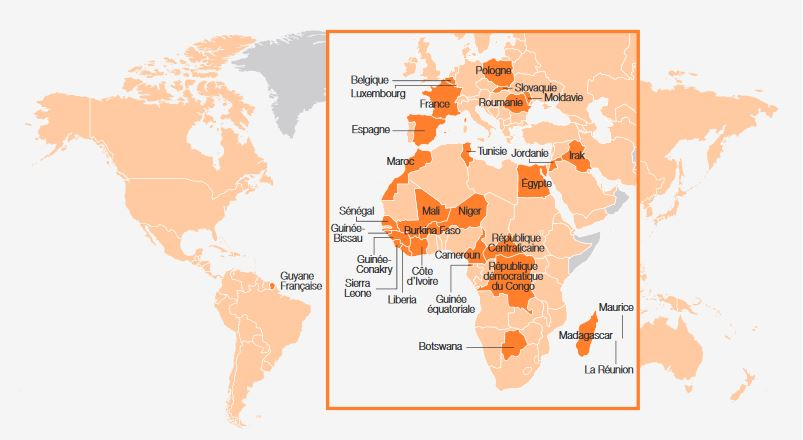
\includegraphics[width=1\textwidth]{./images/implem-mondiale-orange.jpg}
            \caption{Implantation mondiale d'Orange en 2017}
        \end{figure}

        Pour le grand public, l’entreprise est présente dans 29 pays sous la marque Orange avec 6 500 boutiques en nom propre.
        Sa zone de chalandise est l’Europe, l’Afrique et le Moyen-Orient.
        Néanmoins en terme de valeur, la France représente un peu moins de la moitié du chiffre d’affaires, quand l’Afrique et le Moyen-Orient constituent 12 \%.

        \subsubsection{Ses résultats financiers}

        \begin{figure}[!ht]
            \center
            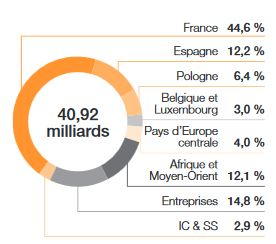
\includegraphics[width=0.4\textwidth]{./images/ca-orange.jpg}
            \caption{Chiffre d'affaires d'Orange Group en 2016}
        \end{figure}

        En 2016, Orange a généré un chiffre d’affaire de près de 41 milliards d’euros.
        L’entreprise en a tiré un résultat net de plus de 3 milliards d’euros et a distribué un dividende de 0,60 euros par action à ses actionnaires.

        \subsubsection{Les ressources humaines}

        Chez Orange se côtoie des fonctionnaires et des salariés sous contrat de droit privé.
        Les premiers sont issus des grandes vagues de recrutement du début des années 1980 pour faire face au retard de déploiement du réseau téléphonique.
        La privatisation de l’entreprise a généré chez eux des dégâts sociaux importants.
        Après des années de déni, la politique des ressources humaines s’est adaptée pour prendre en compte le bien être des salariés.
        Aujourd’hui Orange vise une proportion de 90 \% d’employés recommandant en tant qu’employeur en 2018.
        Fin 2016, ils étaient déjà 88 \% en France.
        Les fonctionnaires représentent encore une grande partie des salariés et sont proches de la retraite ce qui entraîne des départs à la retraite massifs.

        Orange emploie directement 155 000 personnes au 31 décembre 2016, dont 96 000 en France.
        L’entreprise est aussi engagée dans la formation avec le recrutement de 4 300 nouveaux alternants en 2016.

    \subsection{La DSI et ses objectifs}

    La Direction des Systèmes d’Information prend place au sein d’orange France.
    Elle œuvre au bon fonctionnement des différents systèmes d’information du groupe qui sont tous interconnectés pour former un SI\,\footnote{SI : Système d'information.} global.

    La principale mission de la DSI\,\footnote{DSI : Direction des systèmes d'information.} est l’uniformisation et l’évolution de ce SI global qui est un agrégat complexe, résultat des fusions et héritages des technologies commercialisées par le groupe.
    Ce SI est constitué de parties historiques et très hétérogènes ce qui représente une contrainte majeure dans sa maintenance et son fonctionnement tant sur le plan technique que sur le plan financier.
    La complexité du SI est un ensemble de risques, de coûts et de délais qu’il faut réussir à contrôler.

    Le groupe Orange adopte aujourd’hui une stratégie orienté vers les services, la santé et la réactivité de son système d’information sont donc cruciaux.
    La DSI est le cœur stratégique pour permettre au groupe de rester un acteur majeur dans la course à l’innovation et répondre aux attentes du marché d’aujourd’hui comme de demain.

    Une des missions perpétuelle au sein de la DSI est l’urbanisation du SI, cela consiste à  «cartographier» les différents processus métiers pour y répondre de la meilleure façon en diminuant les coûts d’exploitation associés.
    L’urbanisation est la transformation continue du SI pour rester cohérent avec les différents métiers et les stratégies du groupe.
    Cette démarche d’urbanisme permet la réduction des facteurs qui surviennent avec la complexité grandissante d’un système d’information.

    La direction des systèmes d’information est composé d’une entité pas branche métier du groupe ainsi qu’une entité globale qui s’occupent des projets qui portent sur l’ensemble du Si, de façon transverse à plusieurs domaines métiers.

    La DSI est en général la maîtrise d'ouvrage de l'informatique dans le groupe et parfois la maîtrise d'œuvre puisque elle est le centre de décision et l’initiateur des nouveaux projets pour le SI.
    Dans les autres cas la direction des systèmes d’information supervise les projets et est adjoint tant à la maîtrise d’œuvre qu’a la maîtrise d’ouvrage pour s’assurer du respects de ces directives et puisque le pôle architecture est une entité fille de la DSI.

    \subsection{Le pôle architecture et ses missions}

    Le pôle architecture est un centre de compétence de la direction des systèmes d’information.
    L’objectif d’un centre de compétences consiste à regrouper des connaissances : du savoir au savoir-faire autour d’une technologie, d’un outil ou d’une application.
    Selon le périmètre choisi, le centre de compétence interne pourra être responsable des études techniques et de l'intégration des nouveaux projets relatifs à son expertise, réaliser de la veille technologique, être l'interlocuteur de référence face aux intégrateurs et aux éditeurs, émettre de la documentation et formaliser le référentiel du projet, ou assurer le support et l'administration.

    Chez Orange, il existe par exemple un centre de compétence sur les environnements micro-services\,\footnote{Les micro-services sont un style d'architecture particulier se basant sur les API REST et où tout est découplé au maximum.}\,\up{\cite{microservices}} et l’application Docker\,\footnote{Docker est un logiciel plateforme de container, un container ressemble à une machine virtuelle allégée ne contenant que l'application souhaitée et ses dépendances.}\,\up{\cite{docker}} qui permettent une meilleure intégration des applications dans le SI.
    On trouve aussi un centre de compétence autour de la démarche Agile ou un autre plus vaste que les deux exemples précédents : le Pôle architecture, qui regroupe les différents architectes du groupe.

    Ces centres de compétences peuvent dépendre d’un domaine métier ou directement de la direction des systèmes d’information.
    Au sein d’Orange, l’appartenance d’un centre à une entité va dépendre de la manière dont elle a vu le jour.
    Les centres sont référencés dans le SI afin que les acteurs puissent les trouver et y faire appel de façon simple.

    La DSI contient donc le pôle architecture, un regroupement de plus de 600 personnes qui œuvrent au choix et stratégies à propos des applications et du système d’information du groupe.
    Le directeur de l’architecture du SI est Jean-Daniel Guedj qui manage donc ce centre de compétence.
    Le pôle architecture est le regroupement des personnes dont le travail est d’être référent sur les problématiques d’architecture logicielle, d’architecture fonctionnelle et d’architecture technique.

    Plusieurs missions et projets dont la portée est globale au niveau du groupe, et donc transverse à tous les domaines métiers, prennent place dans ce pôle architecture comme par exemple le programme api.
